\chapter{Statistical Models for heterogeneous age groups}
With a full development of statistical rate models for a single age
group behind us, this section turns to a peculiar feature of
population rate meta-analysis: the wide variety of age groups reported
in the literature.

\section{Introduction}
A typical example of the heterogeneity in age groups is shown in
Figure~\ref{age-group-model-af-age-groups}.  The middle of the
age group is scattered against the width of the age group.  Simply
put, there is no standard set of age groups for epilepsy research, and
different studies report results with different age
groups. Unfortunately, this phenomenon is far from unique to epilepsy.

\begin{figure}[h]
\begin{center}
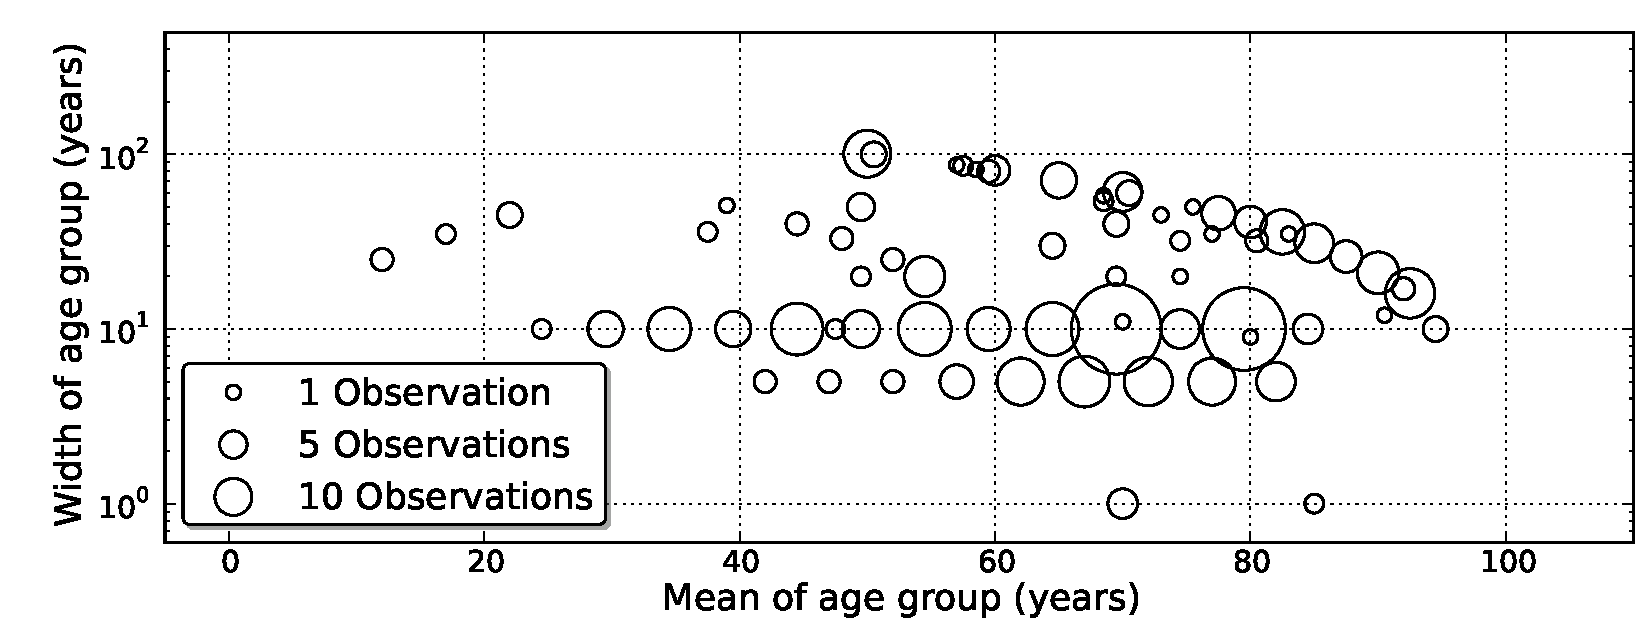
\includegraphics[width=\textwidth]{af_age_groups_scatter.pdf}
%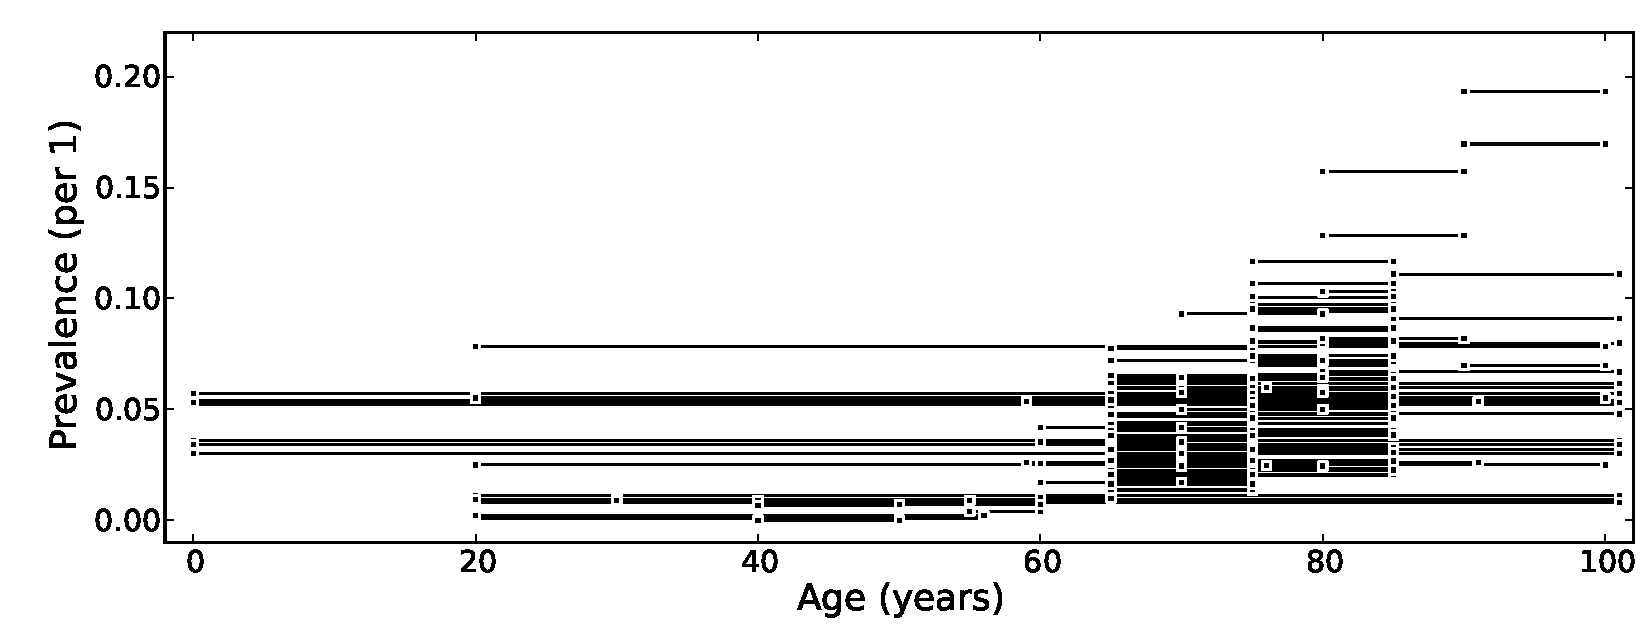
\includegraphics[width=\textwidth]{af_ages_intervals.pdf}
\end{center}
\caption{Mean and spread of age groups in the prevalence data
  collected from a systematic review of atrial fibrilation. The
  size of the circle shows how many observations of this age group
  were found in systematic review. There were
  $586$ rows of prevalence data
  extracted, but the most common age group accounted for only
  $68$ rows.}
\label{age-group-model-af-age-groups}
\end{figure}

This variation in reporting would not be problematic if I had access
to the microdata from all of the systematic review studies.  For
example, using microdata from a national health information system or
from a demographic household survey, I could simply tally the
prevalence rates by single-year age groups.  Although each individual
rate gathered in this way would have high variability, the rate model
from the last section combined with the spline-based age pattern model
from Section~TK would work to produce a combined estimate that is as
uncertain as it should be.

Re-analysis from microdata is occasionally implemented in a GBD study,
however it is often not an option.  I expect the use of microdata
re-analysis to become more frequent when in national and subnational
settings.  In the more common situation where rate microdata is not
available, the rates cannot be re-tallied into homogeneous age groups,
and an alternative approach is needed.

There are several statistical approaches which I have considered, and
they will be compared and contrasted in this section.  Before getting
into this, however, it is worthwhile to examine some of the common
types of age grouping that arise in systematic review.

In the design and dissemination of a study which includes descriptive
epidemiological measurements of population health, there are many
factors that influence the decision of what age groups to include in
analysis.  The authors of each study have often given careful
consideration to the timeless question of scientific research: ``who
do you want to convince of what?''  And the answer often has bearing
on what age groups are appropriate. TK specific examples. Perhaps age
groups were selected before the study was conducted based on a power
calculation, to be wide enough so that the results can claim
statistical significance.  Perhaps there is a scientific hypothesis
about a risk factor or treatment for the condition of interest and the
study was designed to investigate this hypothesis only for an age
group that seemed most likely to shed light on the tangentially
related question of interest.  Even in a study specifically designed
to measure the age pattern of an epidemiological rate, the age groups
may be selected in an ad hoc manner, based on what researchers running
the study think will be most important or communicative.

Regardless of the factors influencing the decision, there is a simple
mathematical model of what is going on.  The study conducts some sort
of measurement on a population of individuals who are all of different
ages, and then the epidemiological rate or rates of interest are
tallied for age groups selected in some context dependent manner. TK
short rant about using half-open intervals to represent age groups
precisely (TK a note on interval notation, and the way this differs
from traditional demography notation, and how my way will be better
once the reader gets used to it.) If the study was a prevalence
study using a full census sample, for example, and if I use
$r_{a_0,a_1}$ to denote the rate for age group $(a_0, a_1)$ and
  $n_{a_0,a_1}$ to denote the subpopulation size of age group
  $(a_0,a_1)$, then the identity
\[
n_{a_0, a_2} = n_{a_0,a_1} + n_{a_1,a_2}
\]
says nothing more complicated than that the size of the subpopulation
of age at least $a_0$ and less than $a_2$ is the sum of the size of
the subpopulation between age $a_0$ and $a_1$ and the size of the
subpopulation between age $a_1$ and $a_2$.  Applying the same
observation to the part of these subpopulations who have the condition
of interest yields the following identity
\[
r_{a_0,a_2} = r_{a_0,a_1}n_{a_0,a_1}/n_{a_0,a_2} + r_{a_1,a_2}n_{a_1,a_2}/n_{a_0,a_2}. 
\] 
In a limiting case of an very large population with very fine age
intervals, this becomes
\[
r_{a_0,a_2} = \int_{a=a_0}^{a_2} r_{a,a+da}n_{a,a+da}/n_{a_0,a_2}\d a
\]
Undoubtedly all real studies are more complicated than this full
census of prevalence, but this is a starting point for conceptualizing
where age-grouped rates come from.  Roughly, they are integrals over
instantaneous rates for infinitesimal age groups.

\section{Overlapping age group data}
\label{theory-age_group_model-overlapping_data}
This section explores several examples of overlapping age group data
collected in systematic reviews, through graphical statistics.  The
primary way I like to display overlapping age-group data is shown in
Figure~\ref{theory-age_group_model-dismod_data_plot}, as horizontal
lines on a plot of age versus rate value.  The level of the bars shows
the rate value, while the width of the bars shows the range of ages
included in the age group. It is often informative to augment these
lines with error bars, showing the uncertainty reported for each rate
value, but for this section I have left out the representation of
uncertainty, to keep the plots as simple as possible.

\begin{figure}[ht]
\begin{center}
\includegraphics[width=\textwidth]{epilepsy_ages_intervals.pdf}
\caption{The systematic review of the descriptive epidemiology of
  epilepsy included $79$ observations of disease prevalence for USA
  with start year before 2000. The prevalence level and age group of
  each observation is shown above as a horizontal bar, with the
  position of the bar along the y-axis representing the prevalence
  level, and the endpoints along the x-axis representing the start and
  end of the age group.  The data shows heterogeneity by age that is
  typical for these systematic review results, appearing to increase
  with age from the teens through adulthood, but with an unclear trend
  at younger and older ages.  }
\label{theory-age_group_model-dismod_data_plot}.
\end{center}
\end{figure}

Each of the horizontal lines in
Figure~\ref{theory-age_group_model-dismod_data_plot} can be
represented as a triple $({a_s}_i, {a_e}_i, r_i)$, where $a_s$ is the
starting age of the age group, $a_e$ is the ending age of the age
group, and $r_i$ is the rate observed for this age group.

A brief word about ${a_e}_i$ is in order here.  Often in the
epidemiological literature, the ending ages are described in a
unit-dependent fashion, for example age group 10-14.  This is intended
to mean from the first day of age 10 to the last day of age 14.
However, this notation can be a hindrance when dealing with age
resolution finer than 1 year, a situation that comes up when studying
neonatal conditions.  For this reason, I prefer the approach that
takes the end age of the interval to be the first age where an
individual is no longer part of the group.  In the case above, I would
say ${a_e}_i = 15$.

Figure~\ref{TK} shows the age group data for a collection of other
condition/area/sex/year combinations.

\begin{figure}[ht]
\includegraphics[width=2in]{TK.pdf}
\caption{TK figures for different conditions
}
\label{theory-age_group_model-dismod_data_plot-multiple}.
\end{figure}


With a firm understanding of the sort of overlapping age group data
that arises in systematic review, I now turn to developing and
analyzing a series of models for the meta-analysis of the data.  There
are five that I will consider: the midpoint model, the disaggregation
model, the midpoint-with-covariate model, the age-standardizing model,
and the age-integrating model.  The age-standardizing model is the
balance of theoretical foundations, practical implementability, and
empirical success that I typically use in the second half of this
book.

\section{Midpoint model}

The simplest approach to modeling data with heterogeneous age
intervals, which is often used in practice \cite{TK}, is to apply each
rate measurement to the midpoint of the age group it measured.  This
is trivial operationally, but it is also theoretically justified
through a ``trapazoidal rule'' integration which will be developed
below in concert with a more elaborate approach.

In practice, this approach works quite accurately for modeling a
disease rate which changes slowly as a function of age.  However, it
becomes quite inaccurate when modeling rates which change more
rapidly.  The typical setting in applications in the second half of
this book will include a few studies which focus on age patterns and
hence have narrow age groups, together with a lot of other studies
which focus on other aspects of disease epidemiology.  Thus the
relevant setting to consider how these models are inaccurate is where
there are a few small-age-group studies and many large-age-group
studies.

Mathematically, the formulation is as follows: let $\boldmu(a)$ be the
spline model of an age-specific rate from Section~TK, and let
$\dens(r,n\given \pi, \rho)$ be the negative binomial rate model from
Section~TK.  Then the likelihood of an observation of rate $r_i$ with
effective sample size $n_i$ for age group $({a_s}_i, {a_e}_i)$ is
simply $\dens\left(r_i, n_i \given
\boldmu\left(\frac{{a_s}_i+{a_e}_i}{2}\right),
\rho\right)$. Equivalently, in ``blackboard notation'', using
$\NBRate(\pi, \rho)$ to denote the negative binomial rate model
distribution, I can write
\begin{align*}
r_i, n_i &\sim \NBRate\left(\boldmu(a_i), \rho\right),\\
a_i &= \frac{{a_s}_i+{a_e}_i}{2}.
\end{align*}
This formulation will be convenient for comparison with the other models of age groups to come.

\begin{figure}[h]
\begin{center}
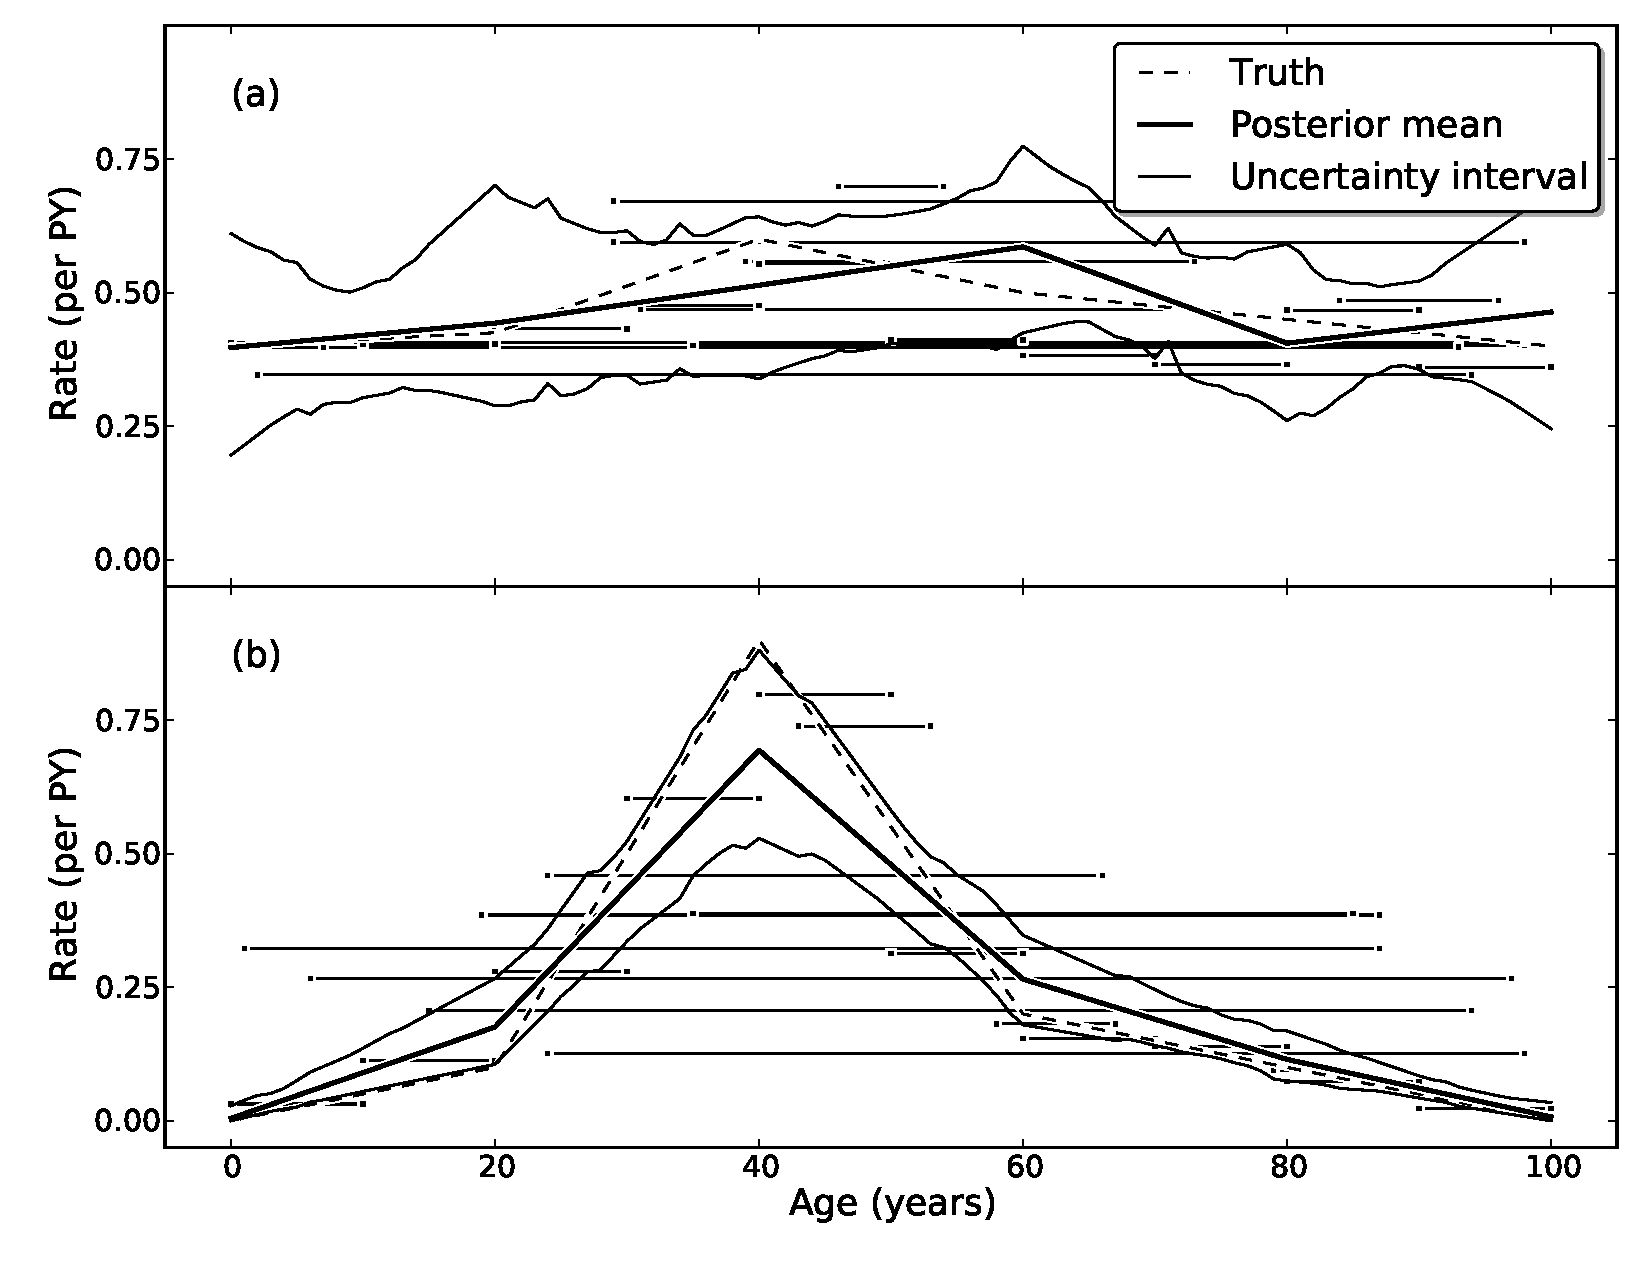
\includegraphics[width=\textwidth]{age_group_midpoint.pdf}
\caption{The midpoint model is a conceptually simple approach to
  dealing with data with heterogeneous age groups, which simply
  attributes the observation to the midpoint of the age group.  Panel
  (a) shows the model applied to an age-specific rate that does not
  vary a great deal across ages, for which the midpoint model is a
  good fit.  Panel (b) shows the model applied to an age-specific rate
  that varies more, for which the midpoint model over-compresses the
  estimates.}
\label{TK-midpoint}
\end{center}
\end{figure}

\section{Disaggregation}
An alternative to the midpoint model which seems appealing but has
some downsides is what I call \emph{disaggregation}.  To understand
the disaggregation approach, imagine the simple re-analysis that I
could do if microdata were available (as described at the beginning of
this chapter).  If I had access to the individual measurements that
went into the calculation of the disease rate found in systematic
review, I could do a re-analysis with any age grouping I wished. I
could calculate rates for single-year age groups, and be sure that the
age pattern is not changing substantially during the grouping.

The microdata from rates found in systematic review are rarely
available, however. The disaggregation approach is a simple attempt to
impute what the rates for the desired age grouping would be \emph{if}
the microdata were available. This requires taking into account the
increased variation that would be found if a study of the same size
was reported for finer age groups.

Without any additional information, rate data reporting a level of $r$
for a population of size $n$ for age group $(a_s,a_e)$, i.e.,
\[
X = (r, n, a_0, a_1)
\]
can be disaggregated into $A = a_e-a_s$ rows of
data, $X_1, X_2, \ldots, X_A$, with 
\[ 
X_a = \left(r, \frac{n}{a_1-a_0}, a, a+1\right), \text{for } a=1,2,\ldots,A. 
\]

Disaggregation can be interpreted as a data preprocessing step, and
this disaggregated data can be fed to the midpoint model from the
previous section to produce a comprehensive estimate of the rate as a
function of age. However, this model has some unintended negative
features when large age intervals are disaggregated.  Because it
ignores the correlation in age of disease levels, it tends to
over-compress age patterns at young and old ages, as shown in Figure~\ref{disagg}.

\begin{figure}[h]
\begin{center}
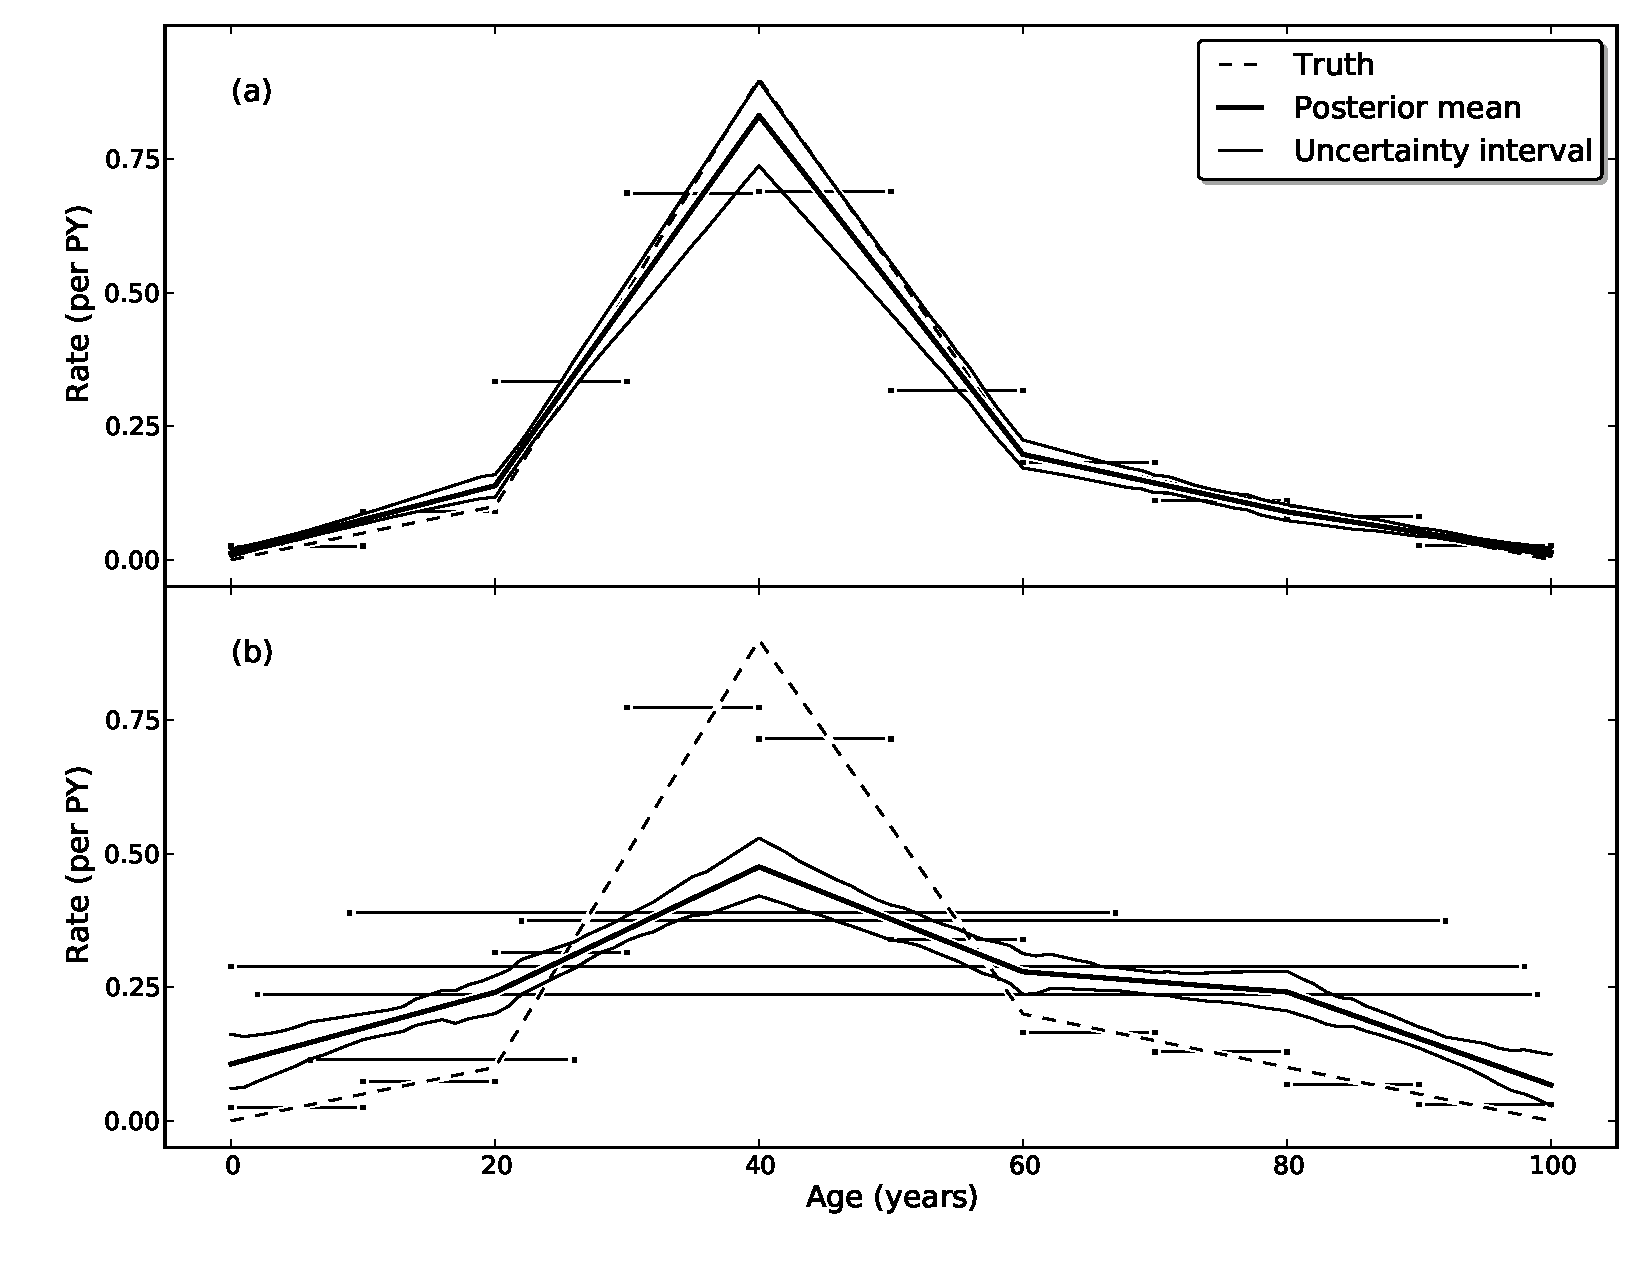
\includegraphics[width=\textwidth]{age_group_disagg.pdf}
\caption{This figure shows the effects of fitting a model with this
  disaggregation approach to the same simulated data shown in the
  midpoint example above.  When the age groups are sufficiently
  fine-grained and homogeneous, disaggregation is a successful
  approach.  But with even slight heterogeneity (Panel b), the model
  estimates are over-compressed}
\label{disagg}
\end{center}
\end{figure}


\section{Midpoint model with group width covariate}
An alternative method, which I consider more ``statistical'' in its
approach, is to add the width of the age group as a covariate into the
midpoint model.  This model takes the form
\begin{align*}
r_i, n_i &\sim \NBRate\left(\mu_i, \rho\right),\\
\mu_i &= \boldmu\left(\frac{{a_s}_i+{a_e}_i}{2}\right) + \theta (a_e � a_s)
\end{align*}

This addresses the shortcomings of the disaggregation approach
\emph{indirectly}, and the indirect nature has positives and
negatives.  This method does not explicitly connect the large age
interval to the small age interval, but instead allows the data to
inform the relationship.  On the other hand, it posits that the
data-driven relationship between the rates for studies with the same
midpoint but different age groups is a linear relationship. In
contrast, the mathematical model developed at the beginning of this
section for how the rate of an age group is measured, is nonlinear in
a specific and mechanistically known way.
Figure~\ref{midpoint-covariate} shows the results of applying this
model to simulated data.


\begin{figure}[h]
\begin{center}
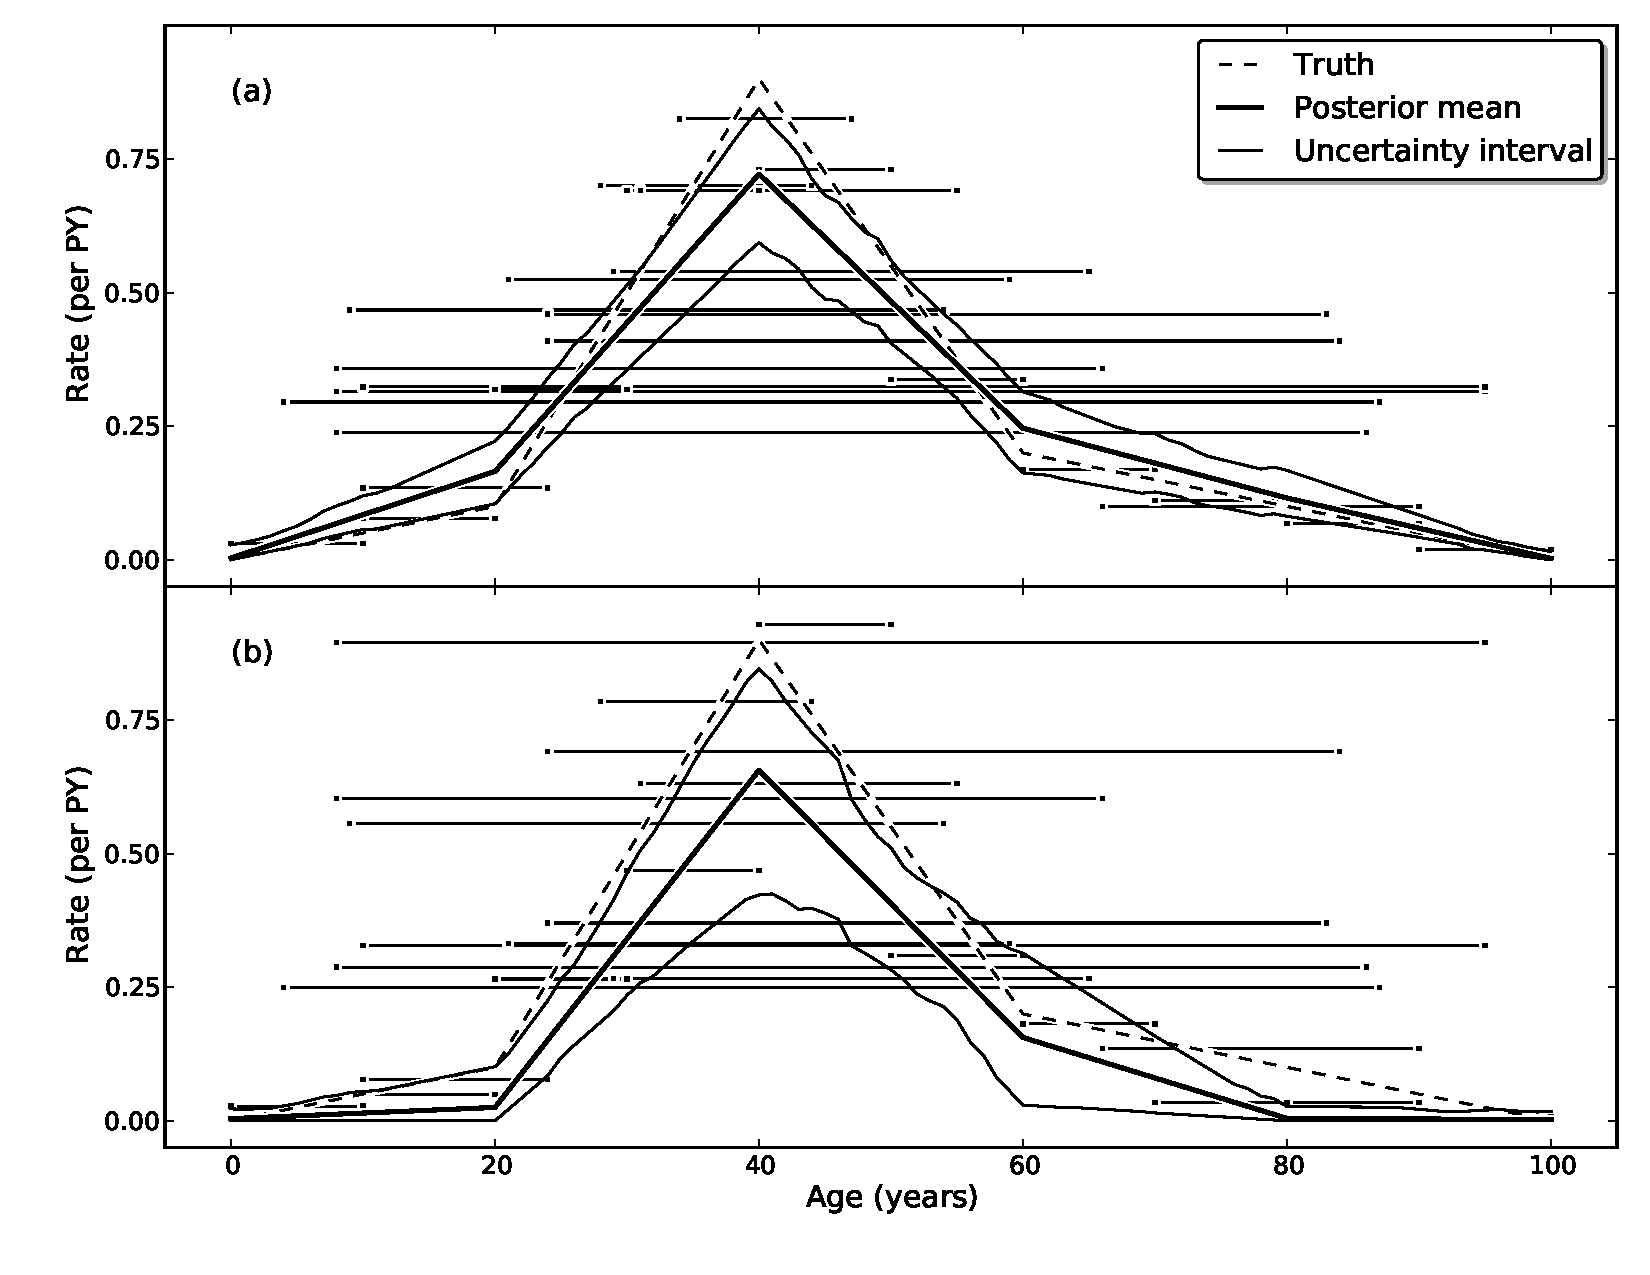
\includegraphics[width=\textwidth]{age_group_midpoint_covariate.pdf}
\caption{TK caption about graphic showing the midpoint covariate model
  at work.}
\label{midpoint-covariate}
\end{center}
\end{figure}

\section{Age-integrating models}
An even more complicated approach, both conceptually and
computationally, is to average across the age interval explicitly in
the statistical model.
\begin{align*}
r_i, n_i &\sim \NBRate\left(\mu_i, \rho\right),\\
\mu_i &= \int_{a=a0_i}^{a1_i} \boldmu(a)\d w(a),
\end{align*}
where the integration $dw$ is weighted according to population
structure.

This has the theoretical appeal of matching the generative model above
by the drawback of being slower to compute and less stable numerically
(to be investigated in detail in Chapter~\ref{TK}).  It also has a
major piece left unspecified, the selection of the age weights for the
integration.  There are two sensible approaches to this, which I call
the \emph{age-standardizing model}, where a common age pattern is used
for all studies and the \emph{age-averaging model}, where the best
estimate available of the age pattern of the study population is used.
The age-standardizing model is faster, due to a computational
optimization to be developed in Chapter~\ref{TK}, but the
age-averaging model is appealing on theoretical grounds, because it
uses the best information available.  However, it is not certain that
using this information will make the end results any more accurate,
because the age pattern of the study population is rarely know with
much certainty, and often it is necessary to assume that it matches
the national age pattern for the country-years where the study was
conducted.  In the case of remission and mortality studies it is even
more complicated to estimate the study population age pattern, since
it is \emph{not} the same as the national population age pattern, but
modulated by the age pattern of disease prevalence.
Figure~\ref{age-group-standardize} shows the results of this model on
simulated data.

\begin{figure}[h]
\begin{center}
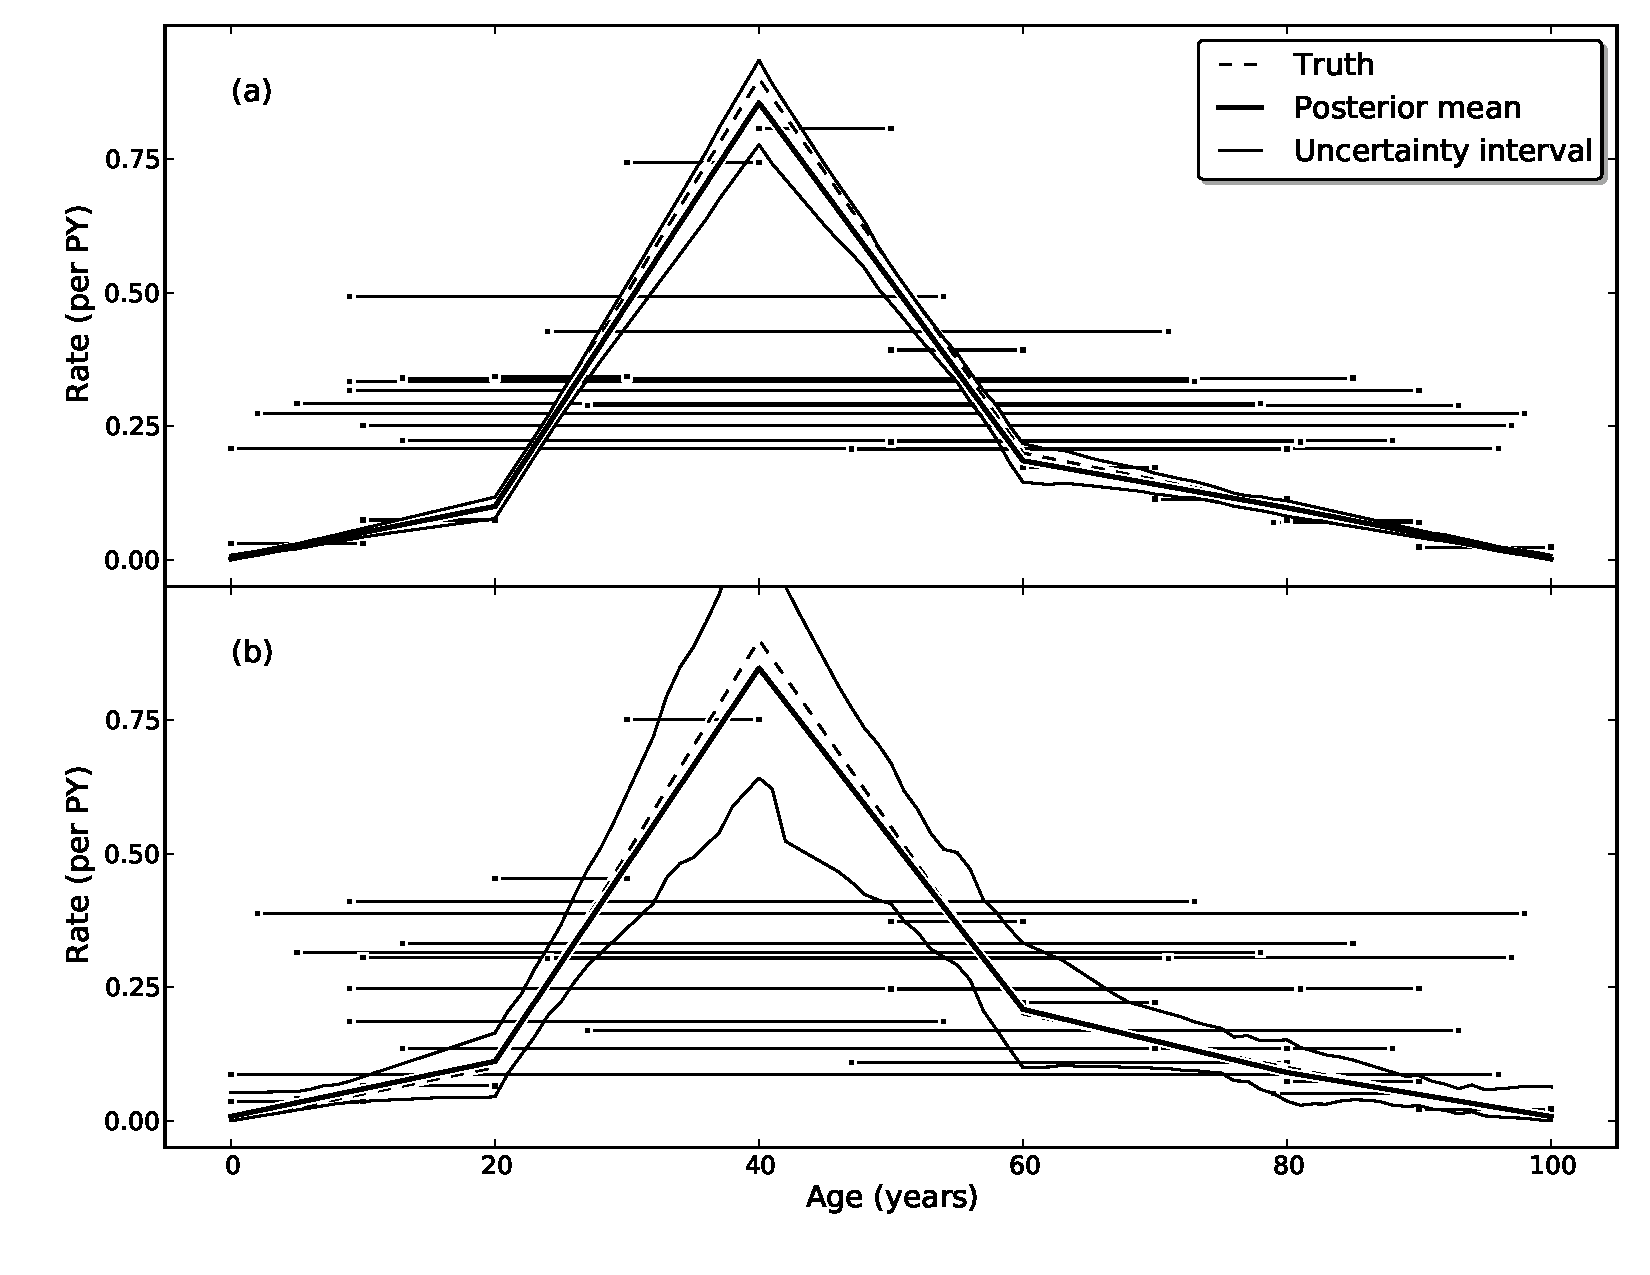
\includegraphics[width=\textwidth]{age_group_standardize.pdf}
\caption{TK caption about Age-standardizing model results in panel (a)
  recover the true age pattern quite precise. Panel (b) shows that the
  results are still accurate when the data generation procedure is
  even more noisy.}
\label{age-group-standardize}
\end{center}
\end{figure}


\section{Model comparison}


\begin{figure}[h]
\begin{center}
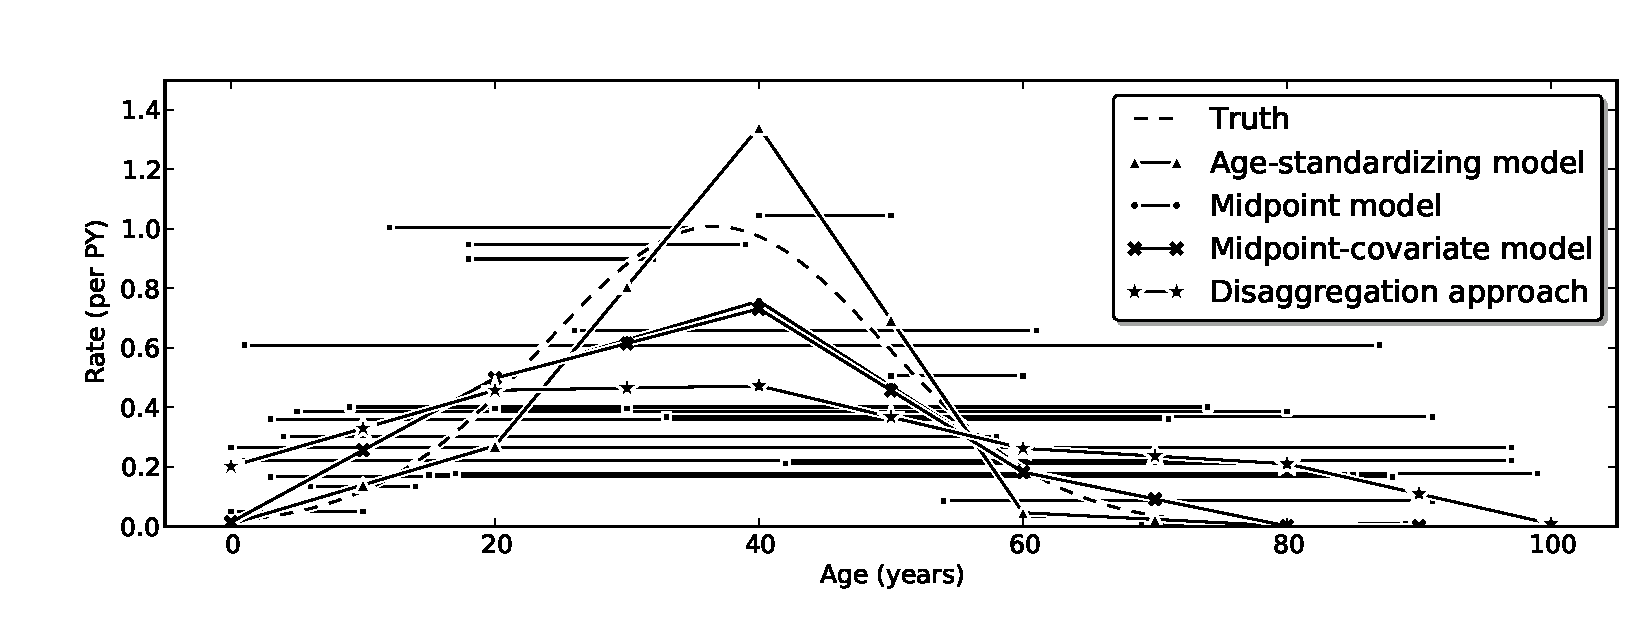
\includegraphics[width=\textwidth]{age_group_models.pdf}
\caption{TK description of this contents of this figure.  }
\label{age-group-model-comparison}
\end{center}
\end{figure}


TK comparison of the various approaches on synthetic data.

An appropriate comparison of these approaches is somewhat difficult to
develop.  One approach is through simulation study, but this risks
inappropriate model selection due to inaccurately choosing the
distribution of the simulated data.  A better approach is
cross-validation, TK description of that I mean by that.  Naively
holding out $25\%$ of the data doesn't address the exact topic of
interest, however, since it determines which model predicts rates of
all age groups, and I am really only interested in predicting the age
groups with small widths accurately.  It would be preferable to hold
out only data with small-width age groups from large representative
subpopulations.  Unfortunately three is rarely enough data to do this,
especially in all the settings that come up in disease modeling.

I have taken a pragmatic approach, evaluating with a variety of
simulations and cross-validations, described now:

TK a description of a combination of approaches:

1) Fit real data to get ``truth''

2) Simulate from truth to get sim data, with random age intervals or with age intervals taken from a real dataset

3) Fit sim data and calculate RMSE and prob cov

Holdout cross-validatoin: Choose 25\% of data to hold out, uniformly
or only from high quality data.  Fit, compare observation and
prediction.

Summary of results: many similarities from all models, although it is
clear that the midpoint model is wrong and the disaggregated midpoint
model is even worse.

For future research, I would like to use cross-validation to select
the best age group model on a case-by-case basis.  This could adapt
the ensemble approach used in CoDMod, where an average of results from
all the different models was computed based on using cross-validation
to decide how much weight each model should be given.

TK results that also include metrics of convergence/algorithmic
stability, showing the superiority of the midpoint model in this
setting.
